\chapter*{\chapterstyle{VII --- Fonctions Vectorielles}} % 95 Fini
\addcontentsline{toc}{section}{Fonctions Vectorielles}

Dans ce chapitre nous étudions les propriétés analytiques et de régularité d'un ensemble plus général de fonctions, les \textbf{fonctions d'une variable à valeurs vectorielles} et plus précisément, on se concentrera principalement sur le cas des fonctions de \(\R\) dans \(\R^n\) muni de sa structure euclidienne si nécessaire.
\subsection*{\subsecstyle{Définition{:}}}
Soit \(A \subset \R\) une partie de \(\R\) et \((f_1, f_2, \ldots, f_n)  \in \mathcal{F}(A, \R)\) des fonctions réelles, alors on appelle \textbf{fonction vectorielle} les fonctions de la forme:
\[
   \begin{aligned}
      f: A &\longrightarrow \R^n\\
      t &\longmapsto (f_1(t), f_2(t), \ldots, f_n(t))
   \end{aligned}
\]
Dans le cas ou \(n = 2\) et si \(\)
\subsection*{\subsecstyle{Limites{:}}}
On caractérise alors \textbf{la limite d'une fonction vectorielle} \(f\) en un point \(a \in A\), par la limite par composante, ie on a:
\[
   \lim_{x \rightarrow a} f(t) = l \Longleftrightarrow \forall i \in \inticc{1}{n} \; ; \; \lim_{x \rightarrow a} f_i(t) = l_i  
\]
En particulier on remarque alors la simplicité de cette généralisation, les limites se calculent simplement composantes par composantes. On verra par la suite que cette définition permet bien d'étendre toutes les notions analytiques classiques.
\subsection*{\subsecstyle{Propriétés de régularité{:}}}
La limite étant caractérisée composantes par composantes, la notion de continuité s'étend naturellement composantes par composantes. Par ailleurs, on étends aussi la notion de dérivabilité et on dit qu'une fonction vectorielle \(f\) est \textbf{dérivable en a} si et seulement si la limite suivante existe:
\[
   \lim_{x \rightarrow a} \frac{f(x) - f(a)}{x - a}
\]
Ce qui équivaut alors à l'existence des limites correspondantes pour les composantes, et \(f\) est donc dérivable en \(a\) (par extension de classe \(\mathcal{C}^k\)) si chacune de ses composantes sont dérivables en \(a\) (ou de classe \(\mathcal{C}^k\) en \(a\)) et on note alors \(f'\) sa \textbf{dérivée} qui s'obtient simplement en dérivant composante par composante.\<

Géométriquement \(f'(t)\) représente \textbf{le vecteur tangent} (aussi appellé vecteur vitesse) à la courbe au temps \(t\). Dans \(\R^2\) par exemple:
\begin{center}
   \begin{tikzpicture}[domain=-2:2, xscale=1.5]
      \tkzInit[xmin=-2,xmax=2,ymin=-2,ymax=2]
      \draw[-latex] (-2,0) -- (2,0) node [right] {$x$};
      \draw[-latex] (0, -2) -- (0,2) node [above] {$y$};
      \draw [thick] plot[color=DarkBlueX, variable=\t, domain=0:2*pi,smooth,thick] ({1.75*sin(2*\t r)},{1.75*sin(3*\t r)});   
      \draw[-Stealth, color=BrightRed1, line width=0.35mm] (1.75, 1.23) -- (1.75,2.2) node [right] {$\;\gamma'(\frac{\pi}{4})$};
   \end{tikzpicture}
\end{center}
\pagebreak
\subsection*{\subsecstyle{Propriétés non-conservées{:}}}
Néanmoins pour l cas de fonctions vectorielles, certaines propriétés ne sont pas conservées. En particulier, \textbf{le théorème de Rolle} n'est plus valable ainsi que le \textbf{le théorème des accroissements finis}.\footnote[1]{Evident aprés un dessin.}
Néanmoins, l'inégalité des accroissement finis reste valide et s'intérprète facilement cinématiquement:
\begin{center}
   \textit{Un point mobile qui se déplace à une vitesse instantanée inférieure à \(K\) sur un temps \(T\), se trouve au maximum à une distance \(KT\) de son point de départ.}
\end{center}
\subsection*{\subsecstyle{Dérivées de composées {:}}}
Soit \(f\) une fonction vectorielle dérivable, on peut alors se demander comment, étant donnée une application linéaire \(L\), se comporte la dérivée de la composée \(L \circ f\) et on montre alors à partir de la définition que:
\[
   (L(f))' = L(f')
\] 
On veut alors généraliser, et on considère deux fonctions vectorielles \(f, g\) dérivables, et une application bilinéaire \(B\), alors de la meme manière on peut montrer que:
\[
   B(f, g)' = B(f', g) + B(f, g')
\]
On peut alors y voir un analogue de la \textbf{règle du produit} pour la dérivation classique, en particulier si \(B = \dotproduct{\cdot}{\cdot}\), on a:
\[
   \dotproduct{f}{g}' = \dotproduct{f'}{g} + \dotproduct{f}{g'}
\]
Finalement, si on a une famille \(f_1, \ldots, f_n\) de fonctions vectorielles dérivables et une application multilinéaire \(M\), alors:
\[
   M(f_1, \ldots, f_n)' = M(f_1', \ldots, f_n) + \ldots + M(f_1, \ldots, f_n')
\]
En particulier si \(M = \det\), et pour les fonctions \(f, g, h\) on a:
\[
   \det(f, g, h)' = \det(f', g, h) + \det(f, g', h) + \det(f, g, h')  
\]
\subsection*{\subsecstyle{Intégration{:}}}
On peut alors raisonnablement penser que l'intégration sur un segment \(\icc{a}{b}\) se généralisera de la meme manière, et c'est le cas ! Si toutes les fonctions \((f_i)\) sont Riemann-intégrables sur le segment, alors on dira que la fonction \(f\) est Riemann-intégrable et on définit:
\[
   \int_{a}^{b} f(t) d t = \left(\int_{a}^{b} f_1(t) d t, \ldots, \int_{a}^{b} f_n(t) d t\right)   
\]
En particulier cela donne lieu à une interprétation cinématique :
\begin{center}
   \textit{Si \(f\) est une fonction qui donne le vecteur vitesse d'un point mobile à un temps \(t\), alors son intégrale est le vecteur position associé.}
\end{center}
\subsection*{\subsecstyle{Points remarquables{:}}}
On peut par la suite définir plus d'outils analytiques sur cet ensemble de fonctions, mais pour cela il faut définir la notion d'arcs paramétré qui nécessite les définitions suivantes qui se ne sont que terminologie:
\begin{itemize}
   \item On appelle \textbf{point régulier} un point \(f(t)\) tel que \(f'(t) \neq 0\)
   \item On appelle \textbf{point critique} un point \(f(t)\) tel que \(f'(t) = 0\)
\end{itemize}
On appelle \textbf{point multiple} un point \(P\) de \(E\) tel qu'il existe \((t_0, \ldots, t_k)\) deux à deux distincts tels que \(\forall i \in \inticc{1}{k} \; f(t_i) = P\) et on appelle alors \textbf{multiplicité} l'entier \(k\).
\chapter*{\chapterstyle{VII --- Fonctions à plusieurs variables}}
\addcontentsline{toc}{section}{Fonctions à plusieurs variables}

Dans ce chapitre nous étudions les propriétés analytiques et de régularité d'un ensemble plus général de fonctions, les \textbf{fonctions d'un espace vectoriel normé dans un autre} et plus précisément, on se concentrera principalement sur le cas des fonctions de \(\R^n\) dans \(\R^p\).\<

Soit \(\mathcal{D}\) une partie de \(\R^n\) et \((x_1, \ldots, x_n) \in \mathcal{D}\), on considère alors la fonction:
\[
   \begin{aligned}
      f : \mathcal{D} \subseteq \R^n &\longrightarrow \R^p \\
      (x_1, \ldots, x_n) &\longmapsto (f_1(x), \ldots, f_p(x))
   \end{aligned}
\]
On dira alors que la fonction \(f_i\) est la i-ème application \textbf{composante} de \(f\).\+

\subsection*{\subsecstyle{Définitions{:}}}
On peut alors définir quelques notions de vocabulaire:
\begin{itemize}
   \item Si la fonction est à valeur scalaire, on dira que c'est \textbf{un champ de scalaires}.
   \item Si la fonction est à valeur vectorielles, on dira que c'est \textbf{un champ de vecteurs}.
\end{itemize}
\subsection*{\subsecstyle{Représentations{:}}}
On cherche alors à représenter de telles fonctions, on sait que dans le cas élémentaire des fonctions à une seule variable, on peut représenter le \textbf{graphe} d'une fonction \(f\) donné par:
\[
   \mathcal{G}_f := \bigl\{ (x, f(x)) \in \R^2 \; ; \; x \in \R \bigl\}   
\]
Dans le cas d'une fonction de plusieurs variables, on peut alors généraliser cette définition par:
\[
   \mathcal{G}_f := \bigl\{ (x, f(x)) \; ; \; x \in \R^n \bigl\}  
\]

De façon générale, le graphe d'une fonction de \(\R^n\) dans \(\R^p\) est un objet à \(n\) dimensions dans l'espace à \((n + p)\) dimensions (les points sont caractérisés par \(n\) paramètres, en termes
savants on dira qu'il s'agit d'une sous-variété de \(\R^{(n + p)}\) de dimension \(n\).\<

Si on considère par exemple une fonction de \(\R^2\) dans \(\R\), c'est alors une fonction qui à chaque point du plan associe une valeur numérique, qu'on peut alors représenter comme \textbf{une hauteur} et on obtient alors \textbf{une surface}, par exemple:

\begin{figure}
   \centering
   \vspace*{-0.5cm}
   \begin{tikzpicture}
      \begin{axis}[domain=-1.5:1.5,y domain=-1.5:1.5, scale=1, colormap={custom}{color(0)=(DarkBlue3) color(1)=(BrightBlue1)}]
        \addplot3[draw=black, opacity=0.5, surf, samples=40] {exp(-x^2-y^2)};
      \end{axis}
    \end{tikzpicture}
   \captionsetup{labelformat=empty}
   \caption{Graphe de la fonction \(f : (x, y) \mapsto \exp(-x^2 - y^2)\)}
\end{figure}
\pagebreak

Dans le cas général néanmoins, il est plus difficile de représenter ce type de fonctions mais on peut par exemple s'inspirer des fonctions \(\C \rightarrow \C\) et utiliser la \textbf{couleur} comme 4-ème dimension de l'image. On peut aussi de manière heuristique représenter simplement le domaine de départ et/ou d'arrivée pour étudier le comportement de la fonction.
\subsection*{\subsecstyle{Cas des champs de vecteurs{:}}}
De manière générale, le caractère multidimensionnel de l'espace d'arrivée importe peu dans tout le chapitre qui va suivre, les notions analytiques étant définies à partir d'une limite, elles passeront aux composantes comme les notions évoquées au chapitre précédent.\<

Dans toute la suite on considèrera alors souvent le cas épuré de champs de scalaires et il est attendu d'adapter les résultat élémentaires aux cas à valeurs vectorielles.
\subsection*{\subsecstyle{Lignes de niveaux{:}}}
On considère une fonction \(f : \R^2 \rightarrow \R\), alors on appelle \textbf{ligne de niveau} associé à la valeur \(\lambda\) l'ensemble suivant:
\[
   L_\lambda := \Bigl\{ (x, y) \in \R^2 \; ; \; f(x, y) = \lambda \Bigl\}   
\]
C'est une courbe plane qui représente l'ensemble des points du plan ou la fonction prends une valeur fixée, tracer plusieurs lignes de niveaux permet alors d'obtenir des informations sur la fonction, par exemple:
\begin{figure}[h]
   \centering
   \begin{tikzpicture}[line cap=round, scale=2]
      \tkzInit[xmin=-2,xmax=2,ymin=-2,ymax=2]
      \draw[-latex] (-2,0) -- (2,0) node [right] {$x$};
      \draw[-latex] (0, -2) -- (0,2) node [above] {$y$};

      \draw [thick, color=BrightRed1] plot[domain=0:2*pi,variable=\t, line width=0.3mm, smooth] ({0.226480229573*cos(\t r)}, {0.226480229573*sin(\t r)});   
      \draw [thick, color=BrightRed2] plot[domain=0:2*pi,variable=\t, line width=0.3mm, smooth] ({0.536360021303*cos(\t r)}, {0.536360021303*sin(\t r)});   
      \draw [thick, color=DarkGreen1] plot[domain=0:2*pi,variable=\t, line width=0.3mm, smooth] ({0.83255461115*cos(\t r)}, {0.83255461115*sin(\t r)});   
      \draw [thick, color=DarkGreen2] plot[domain=0:2*pi,variable=\t, line width=0.3mm, smooth] ({1.17741002252*cos(\t r)}, {1.17741002252*sin(\t r)});   
      \draw [thick, color=DarkGreen3] plot[domain=0:2*pi,variable=\t, line width=0.3mm, smooth] ({1.51742712939*cos(\t r)}, {1.51742712939*sin(\t r)});    
      \draw node[color=BrightRed1] at (0.27, 0.27) {\scriptsize $L_{0.95}$};
      \draw node[color=BrightRed2] at (0.49, 0.49) {\scriptsize $L_{0.75}$};
      \draw node[color=DarkGreen1] at (0.7, 0.7) {\scriptsize $L_{0.50}$};
      \draw node[color=DarkGreen2] at (0.95, 0.95) {\scriptsize $L_{0.25}$};
      \draw node[color=DarkGreen3] at (1.2, 1.2) {\scriptsize $L_{0.10}$};
   \end{tikzpicture}
   \captionsetup{labelformat=empty}
   \caption{Lignes de niveau de la fonction \(f : (x, y) \mapsto \exp(-x^2 - y^2)\)}
\end{figure}
\subsection*{\subsecstyle{Changements de variables{:}}}
L'étude des fonctions à plusieurs variables va nous amener à étudier les \textbf{changements de variables} que nous allons définir:
\begin{center}
   \textbf{On appelle changement de variable tout \(\mathcal{C}^k\) difféomorphisme entre deux espaces.}
\end{center}
En particulier, on verra que le passage en coordonées polaires défini comme suite est bien un changement de variable et en tant que tel, il préserve les propriétés différentielles:
\[
   \begin{aligned}
      \phi : \R_+^* \times \ioo{-\pi}{\pi} &\longrightarrow \R^2 \backslash (\R_- \times \{0\})\\
      (r, \theta) &\longmapsto (r\cos(\theta), r\sin(\theta))
   \end{aligned}
\]
\chapter*{\chapterstyle{VII --- Limite \& Continuité}}
\addcontentsline{toc}{section}{Limite \& Continuité} 
Dans ce chapitre et comme vu dans le chapitre de Topologie, nous étudirons le concept de limite dans le cas d'une fonction à plusieurs variables, plus précisément, sauf exceptions, dans le cas d'un champ de scalaire. Dans les cas ou les généralités sont triviales, on utilisera sans vergogne l'exemple canonique d'une fonction \(f : \R^2 \rightarrow \R\). On rapelle qu'une limite d'une telle fonction se caractérise métriquement par la propriété:
\[
   \forall \epsilon >0 \; , \; \exists \lambda > 0 \; , \; \forall x \in \R^n \; , \; \vectNorm{x - a} < \lambda \implies |f(x) - l| < \epsilon
\]

\subsection*{\subsecstyle{Limites suivant une restriction{:}}}
Cette définition correspond bien à l'intuition \textit{topologique} de la notion de limite. En particulier, on peut alors montrer que si \(f\) tends vers \(l\) en \((a, b)\), alors en particulier si on considère un \textbf{chemin} de la forme:
\[
   \gamma : t \mapsto (\gamma_1(t), \gamma_2(t))   
\]
Et si ce chemin est tel qu'il passe par \((a, b)\) en \(t_0\), alors on a nécessairement:
\[
   \lim_{(x, y) \rightarrow (a, b)} f(x, y) = l \implies \lim_{t \rightarrow t_0} f(\gamma(t)) = l
\]
En particulier cela nous permet de construire une méthode pour démontrer la \textbf{non-existence de limite}, ie:
\begin{center}
   \textit{Si il existe deux chemins différents suivant lesquels la fonction admets deux limites différentes, alors elle n'admet pas de limite en ce point.}
\end{center}
\subsection*{\subsecstyle{Erreurs communes{:}}}
Cette définition correspond bien à l'intuition \textit{topologique} de la notion de limite. Néanmoins il faut remarquer les propriétés suivantes spécifiques aux fonctions à plusieurs variables:
\begin{itemize}
   \item Il est possible qu'une fonction admette une limite suivant plusieurs chemins, mais pas de limite.
   \item Il est meme possible qu'une fonction admette une limite suivant toutes les droites, mais pas de limite.
   \item De manière générale, admettre une limite sur plusieurs restrictions ne permet pas d'affirmer l'existence d'une limite.
\end{itemize}
\subsection*{\subsecstyle{Opérations{:}}}
Comme dans le cas des fonctions réelles, on peut alors démontrer les propriétés opératoires de la limite, en effet si on considère \(f, g\) deux champs scalaires qui admettent deux limites \(l_1, l_2\) en \(A \in \R^p\),alors on a les propriétés suivantes:
\begin{itemize}
   \item Le passage à la limite est \textbf{linéaire}.
   \item Le passage à la limite est \textbf{multiplicatif}.
   \item Le passage à la limite (non-nulle) d'une fonction localement non-nulle est \textbf{inversible}.
\end{itemize}
La première propriété se généralise aux champs vectoriels, mais pas les deux secondes bien évidemment, car les opérations en jeu (effectuées à l'arrivée) ne sont pas définies pour des vecteurs.\<

Enfin pour deux fonction qui sont composables, on a la propriété fondamentale suivante:
\begin{itemize}
   \item Le passage à la limite est compatible avec la \textbf{composition}.
\end{itemize}
\subsection*{\subsecstyle{Théorème d'encadrement {:}}}
On peut généraliser le théorème des gendarmes aux fonctions à plusieurs variables, en effet si on considère \(f, g, h\) trois fonctions telles que \(f(x, y) \leq g(x, y) \leq h(x, y)\) dans un voisinage de \((a, b)\) alors on a:
\[
   \lim_{(x, y) \rightarrow (a, b)} f(x, y) = \lim_{(x, y) \rightarrow (a, b)} h(x, y) = l \implies \lim_{(x, y) \rightarrow (a, b)} g(x, y) = l
\] 
\pagebreak
\subsection*{\subsecstyle{Passage en polaire {:}}}
Si on considère une fonction à deux variables, on peut exprimer \((x, y)\) en coordonées polaires, ie considérer la composée \(f(x, y) = f(r\cos(\theta), r\sin(\theta))\) et alors \(f\) tends vers \(0\) en \((0, 0)\) si et seulement si il existe une fonction \(g(r)\) telle que:
\[
   |f(r\cos(\theta), r\sin(\theta))| \leq g(r)
\]
Avec \(g(r)\) qui tends vers \(0\) quand \(r\) tends vers \(0\). \textbf{Attention} la fonction \(g\) ne doit plus dépendre de \(\theta\).
\subsection*{\subsecstyle{Continuité {:}}}
En tant que conséquence directe de la définition topologique, on dira alors qu'une fonction est \textbf{continue} en un point \(A\) si et seulement si:
\[
   \lim_{(x, y) \rightarrow A} f(x, y) = f(A)   
\]
Et toute les propriétés opératoires usuelles sont alors aisément démontrées. En particulier, on peut montrer que toutes les fractions rationnelles sont continues sur leur ensemble de définition, et donc tout les polynomes.

\chapter*{\chapterstyle{VII --- Dérivées Directionnelles}}
\addcontentsline{toc}{section}{Dérivées Directionnelles} 
Dans ce chapitre nous essaierons de construire un concept de \textbf{dérivée} dans le cas d'une fonction à plusieurs variables, plus précisément, sauf exceptions, dans le cas d'un champ de scalaire. Dans les cas ou les généralités sont triviales, on utilisera sans vergogne l'exemple canonique d'une fonction \(f : \R^2 \rightarrow \R\)

\subsection*{\subsecstyle{Applications Partielles {:}}}
On considère une fonction de \(A \subseteq \R^p \rightarrow \R\) et un point \(a = (a_1, \ldots, a_n)\) \textbf{intérieur} à \(A\). Alors il existe un voisinage de \(a\) ou la fonction \textbf{réelle} suivante est bien définie, on l'appelle alors \textbf{i-ème application partielle} au point \(a\):
\[
   \begin{aligned}
      f_{x_i} : \R &\longrightarrow \R\\
      t &\longmapsto f(a_1, \ldots, t, \ldots, a_n)
   \end{aligned}
\]
\begin{center}
   \textit{Considèrer la i-ème application partielle, c'est fixer une direction et considèrer la courbe de \(f\) suivant cette direction.}
\end{center}
Géométriquement, on peut le voir comme l'interesection d'un plan parallèle à l'axe considéré et passant par \(a\), et l'application partielle est alors l'intersection de la courbe et du plan:
\begin{figure}[h]
   \centering
   \begin{tikzpicture}
      \begin{axis}[domain=-1.5:1.5,y domain=-1.5:1.5, scale=1, colormap={custom}{color(0)=(DarkBlue3) color(1)=(BrightBlue1)}]
         \addplot3[draw=black, opacity=0.5, surf, samples=40] {exp(-x^2-y^2)};
         \addplot3[draw=DarkBlueX, line width = 0.5mm, samples=51, samples y=0,domain=-1.5:1.5,variable=\t]
         ({\t},{-0.5},{exp(-\t^2 - 0.5^2)});         
      \end{axis}
    \end{tikzpicture}
   \captionsetup{labelformat=empty}
   \caption{Application partielle \(f_x\) en \((0, -0.5)\) de \(f : (x, y) \mapsto \exp(-x^2 - y^2)\)}
\end{figure}
\subsection*{\subsecstyle{Dérivées Partielles {:}}}
On dira alors qu'une telle fonction \textbf{admet une i-ème dérivée partielle} au point \(a\) si et seulement si sa i-ème application partielle en \(a\) est dérivable en \(a_i\). On se ramène alors à l'étude de la dérivabilité d'une fonction \textbf{réelle}, ce qui ne pose pas de problème théorique. Dans ce cas, on notera alors:
\[
   \frac{\partial f}{\partial x_i}(a) = f_{x_i}'(a_i)   
\]
Si \(f\) admet une i-ème dérivée partielle sur un ouvert \(\mathcal{U}\) si et seulement si elle en admet en tout points de \(\mathcal{U}\) et on définit alors:
\[
   \begin{aligned}
      \frac{\partial f}{\partial x_i} : \mathcal{U} &\longrightarrow \R\\
      a &\longmapsto \frac{\partial f}{\partial x_i}(a_i)
   \end{aligned}
\]
On dira alors qu'un fonction à plusieurs variables est de classe \(\mathcal{C}^k\) en un point si elle admet toutes ses dérivées partielles en ce point et qu'elles y sont continues.
\pagebreak
\subsection*{\subsecstyle{Propriétés opératoires{:}}}
On peut montrer que la dérivation partielle est un \textbf{opérateur différentiel} agissant sur un espace de fonctions qui admettent des dérivées partielles, en particulier en utilisant les définitions précédentes et en notant \(\mathcal{D}_i(\R^n)\) l'espace des fonctions admettant une i-ème dérivée partielle, alors on peut définir:
\[
   \begin{aligned}
      \frac{\partial}{\partial x_i} : \mathcal{D}_i(\R^n) &\longrightarrow \mathcal{F}(\mathcal{U}, \R)\\
      f &\longmapsto \frac{\partial f}{\partial x_i}
   \end{aligned}
\]

C'est donc cet opérateur que nous appliquons à une fonction qui admet des dérivées partielles. En particulier, l'intéret de cette définition est alors de pouvoir affirmer les propriétés suivantes:
\begin{itemize}
   \item La dérivation partielle est \textbf{linéaire}.
   \item La dérivation partielle suit \textbf{la règle du produit}.
\end{itemize}
La première propriété se généralise aux champs vectoriels, mais pas la seconde bien évidemment, car les opérations en jeu (effectuées à l'arrivée) ne sont pas définies pour des vecteurs.\<

\underline{Exemple:} On considère les fonctions suivantes en un point \((x, y)\):
\[
   \begin{aligned}
      f : (x, y) &\longmapsto xy \quad\quad\quad g : (x, y) &\longmapsto x^2y
   \end{aligned}
\]
Alors on a\footnote[1]{\textbf{Attention:} Ici on fait l'abus de notation usuel d'utiliser deux fois la variable \(x\) qui ont deux sens différents, l'expression \(\partialD{fg}{x}\) signifie simplement qu'on dérive par rapport à la première variable (penser \(\partial_1(fg)\)) et \((x, y)\) représente le point d'évaluation de la dérivée partielle.)}:
\[
   \partialD{(fg)}{x}(x, y) = \partialD{f}{x}(x, y)g(x, y) + \partialD{g}{x}(x, y)f(x, y) = yx^2y + 2xyxy = 3x^2y^2
\]
On voit bien ici que la dérivée d'un produit n'a de sens que si on est dans le cas de (au moins un) champs scalaires !
\subsection*{\subsecstyle{Dérivée partielle d'une composée{:}}}
Le cas de la composée est plus subtil et on reviens temporairement au cas général des deux champs vectoriels suivants dont on supposera qu'ils admettent toutes leurs dérivées partielles partout:
\[
   \begin{aligned}
      g : \R^m &\longmapsto \R^n \quad\quad\quad f : \R^n &\longmapsto \R^p
   \end{aligned}
\]
On cherche à caculer la dérivée partielle par rapport à la \(i\)-ème variable de la fonction \(f \circ g\) au point \(a\), on peut alors montrer la formule suivante, appellée \textbf{chain rule}: 
\[
   \partialD{(f \circ g)}{x_i}(a) = \sum_{k=1}^{n} \partialD{g_k}{x_i}(a)\partialD{f}{x_k}(g(a))
\]
\underline{Exemple:} On considère un fonction \(f : \R^2 \rightarrow \R\) de classe \(\mathcal{C}^1\) et la fonction \(g\) de passage en polaire:
\[
   \begin{aligned}
      g : (r, \theta) &\longmapsto (r\cos(\theta), r\sin(\theta))
   \end{aligned}
\]
On se propose de calculer la première dérivée partielle de \(f \circ g\) au point \((r, \theta)\), on a alors:
\begin{flalign*}
   \partialD{(f \circ g)}{r}(r, \theta) 
   &= \partialD{g_1}{r}(r, \theta)\partialD{f}{x}(r\cos(\theta), r\sin(\theta)) + \partialD{g_2}{r}(r, \theta)\partialD{f}{y}(r\cos(\theta), r\sin(\theta))\\ 
   &= cos(\theta)\partialD{f}{x}(r\cos(\theta), r\sin(\theta)) + sin(\theta)\partialD{f}{y}(r\cos(\theta), r\sin(\theta))
\end{flalign*}
\subsection*{\subsecstyle{Dérivées partielles d'ordre supérieur {:}}}
La i-ème dérivée partielle de \(f\) étant à nouveau une fonction de \(n\) variables, on peut alors considèrer ses dérivées partielles. On définit les dérivées partielles secondes de \(f\) (si elles existent), notées:
\[
   \frac{\partial^2 f}{\partial x_i \partial x_j}(a)   
\]
Et par récurrence les dérivées partielles d'ordre \(k\) par:
\[
   \frac{\partial^k f}{\partial x_{i_1} \ldots \partial x_{i_k}}(a)
\]
Et on se pose alors la question de l'importance de \textbf{l'ordre de dérivation} et de manière générale, on peut alors montrer que l'ordre d'application de l'opérateur compte, ie que:
\[
   \frac{\partial^2 f}{\partial x_j \partial x_i}(a) \neq \frac{\partial^2 f}{\partial x_i \partial x_j}(a)
\]
Mais le théorème de Schwarz donne alors une condition suffisante pour que l'ordre ne compte pas:
\begin{center}
   \textbf{Si les dérivées partielles sont toutes continues en un point, alors l'ordre de dérivation n'importe pas.}
\end{center}
\subsection*{\subsecstyle{Dérivées Directionnelles {:}}}
Si on considère les dérivées partielles d'une fonction \(f\), qu'on note \(a = (x_1, \ldots, x_n)\) le point d'étude et \((e_i)\) la base canonique, on peut alors les caractériser par:
\[
   \frac{\partial f}{\partial x_i}(a) = \lim_{h \rightarrow 0} \frac{f(a + he_i) - f(a)}{h}
\] 
En effet ce sont par définition les dérivées des applications partielles, donc des limites de taux d'accroissement\footnote[1]{Cette limite n'étant pas trés pratique pour des calculs concrets, on verra au chapitre suivant une caractérisation plus utile dans le cas de fonctions différentiables.} qui correspondent à la limite ci-dessus.\+
Ce sont en fait des \textbf{dérivées directionnelles} dans des directions canoniques, mais on souhaite alors généraliser cette notion à tout vecteur unitaire \(v\), on pose alors simplement:
\[
   D_vf(a) = \lim_{h \rightarrow 0} \frac{f(a + hv) - f(a)}{h}
\]
\begin{center}
   \textit{C'est alors intuitivement la dérivée de la courbe obtenue par intersection avec le plan vertical suivant le vecteur choisi.}
\end{center}

\subsection*{\subsecstyle{Inconvénients de cette définition{:}}}
On aimerait alors que cette définition remplisse les memes roles que ceux remplis par la dérivée usuelle, mais ce n'est pas du tout le cas, en particulier, on a les problèmes suivants:
\begin{itemize}
   \item Un fonction qui admet des dérivées partielles en un point peut ne pas etre continue en ce point.
   \item Un fonction qui admet toute ses dérivées directionnelles en un point peut ne pas etre continue en ce point.
   \item Elles ne permettent pas directement de définir une application affine tangente à la courbe.
   \item Elles ne permettent pas d'étudier les extrema de la fonction.
\end{itemize}
\begin{center}
   \textit{En résumé, le concept de dérivée directionnelle manque de puissance.}
\end{center}
\chapter*{\chapterstyle{VII --- Différentielle}}
\addcontentsline{toc}{section}{Différentielle} 
Nous allons à présent définir le vrai concept équivalent à la dérivée usuelle, qui nous permettra de généraliser l'idée d'application tangente en un point, d'étudier les extrema d'une fonction et d'étudier toutes les propriétés différentielles d'une fonction à plusieurs variables de manière générale.\<

Dans toute la suite, on s'appropriera la notation suivante des vecteurs de la \textbf{base duale}\footnote[1]{Formellement, il s'agit d'un \textbf{champ de formes 1-linéaire} (on dira aussi \textbf{1-forme différentielle}) qui à chaque point \(a\) de \(\R^n\) associe la projection canonique sur la i-ème coordonée de "l'espace tangent" en \(a\), mais dans ce cas, \(T\R^n = \R^n\), donc le champ de forme linéaire se réduit simplement en une simple forme linéaire (ou plutot un champ constant).} de \(\R^n\):
\[
   \begin{aligned}
      dx_i : (x_1, \ldots, x_n) &\longmapsto x_i 
   \end{aligned}
\]
\subsection*{\subsecstyle{Cas réel{:}}}
On rappelle qu'on dit qu'une fonction réelle \(f\) est dérivable en \(a\) de nombre dérivé \(f'(a)\) si et seulement si\footnote[2]{Ce qui est équivalent à dire que \(f(a + h) - f(a) - f'(a)h = o(|h|)\) au voisinage de \(0\)}:
\[
   \forall h \in \R \; ; \; \frac{f(a + h) - f(a) - f'(a)h}{h} \underset{h \rightarrow 0}{\longrightarrow} 0
\]
Cette definition revient alors à dire que l'application linéaire qui approxime le mieux \(f\) en \(a\) est donnée par:
\[
   \begin{aligned}
      df_a : \R &\longrightarrow \R\\
      x &\longmapsto f'(a)dx(x) = f'(a)x 
   \end{aligned}  
\]
Ce qui correspond à dire que la fonction \(df_a(x) = f'(a)x\) est \textbf{l'application linéaire tangente} à \(f\) au point \(a\). Attention, ici on dit bien linéaire, et donc ce n'est pas une tangente géométrique à la courbe, mais son pendant affine l'est.\<

On définit alors la \textbf{différentielle} de \(f\) comme la fonction qui a tout point ou \(f\) est dérivable, lui associe son application linéaire tangente, ie:
\[
   \begin{aligned}
      df : \R &\longrightarrow \mathcal{L(\R, \R)}\\
      a &\longmapsto f'(a)dx
   \end{aligned}  
\]
\begin{center}
   \textit{C'est cette notion de différentiabilité et d'application linéaire tangente qui va se généraliser dans tout sa force au cas général.}
\end{center}
\subsection*{\subsecstyle{Définition{:}}}
Soit \(f : \R^n \rightarrow \R^p\), on dira que \(f\) est \textbf{différentiable} en un point \(a\) si et seulement si il existe une application linéaire \(df_a : \R^n \rightarrow \R^p\) telle que:
\[
   \forall h \in \R^n \; ; \; \frac{f(a + h) - f(a) - df_a(h)}{\vectNorm{h}} \underset{h \rightarrow 0}{\longrightarrow} 0
\]
Ou en d'autre termes qu'il existe \(\epsilon_a\) une fonction définie sur un voisinage de \(0\), telle que \(\epsilon_a(h) \underset{h \rightarrow 0}{\rightarrow} 0\) et que: 
\[
   \forall h \in \R^n \; ; \; f(a + h) - f(a) - df_a(h) = \vectNorm{h}\epsilon_a(h)
\]
En outre, si \(f\) est différentiable sur un ouvert \(U\), alors on définit sa différentielle de la meme manière que dans le cas réel par:
\[
   \begin{aligned}
      df : \R^n &\longrightarrow \mathcal{L}(\R^n, \R^p)\\
      a &\longmapsto df_a
   \end{aligned}  
\]
Mais cette définition ne nous permet pas de connaitre la \textbf{forme} de la différentielle, et donc de la calculer, on doit donc chercher des conditions nécessaires sur cette fonction dans la section suivante. 

\subsection*{\subsecstyle{Forme nécessaire de la différentielle{:}}}
En exprimant les applications partielles de \(f\) et en utilisant la définition de la différentielle appliqué au quotient obtenu, on montre tout d'abord que \(f\) admet nécessairement toutes ses dérivées partielles en \(a\) et on a:
\[
   \partialD{f}{x_i}(a) = df_a(e_i)   
\]
Alors, en exprimant un vecteur \(x \in \R^n\) dans la base canonique et en utilisant la linéarité de la différentielle, on obtient l'expression:
\[
   df_a(x) = \sum_{k=1}^{n}x_i df_a(e_i) = \sum_{k=1}^{n} \partialD{f}{x_i}(a) x_i = \sum_{k=1}^{n} \partialD{f}{x_i}(a) dx_i
\]
Finalement, on a bien donné une forme nécessaire à la différentielle de \(f\) et on a:
\[
   \begin{aligned}
      df : \R^n &\longrightarrow \mathcal{L}(\R^n, \R^p)\\
      a &\longmapsto \sum_{k=1}^{n} \partialD{f}{x_i}(a) dx_i
   \end{aligned}  
\]
C'est bien une application linéaire à valeurs dans \(\R^p\) car par composantes \(\partialD{f}{x_i}(a)\) est un vecteur et le produit \(vdx\) est bien défini car \(dx\) est une forme linéaire.\<

\underline{Exemple:} On considère la fonction \(f : (x, y) \mapsto (xy, x + y)\), dont on souhaite calculer la différentielle en \(a = (1, 1)\) alors on a:
\[
   \begin{cases}
      \partialD{f}{x}(x, y) = (y, 1)\\
      \partialD{f}{y}(x, y) = (x, 1)
   \end{cases}   
\]
Donc la différentielle est donnée par:
\[
   df : (a, b) \mapsto (b, 1)dx + (a, 1)dy
\]
Et donc la différentielle en \(a\) est donnée par:
\[
   df_a : (x, y) \mapsto (1, 1)x + (1, 1)y = (x + y, x + y)
\]

\subsection*{\subsecstyle{Propriétés opératoires{:}}}
Tout d'abord, on peut montrer que \textbf{l'opérateur de différentiation} sur les applications différentiables sur un ouvert \(\mathcal{U}\), qu'on notera \(\mathscr{D}_\mathcal{U}\), est un opérateur différentiel:
\[
   \begin{aligned}
      d : \mathscr{D}_\mathcal{U} &\longrightarrow \mathcal{F}(\mathcal{U}, \mathcal{L}(\R^n, \R^p))\\
      f &\longmapsto df
   \end{aligned}
\]
C'est donc cet opérateur que nous appliquons à une fonction qui admet une différentielle. En particulier, l'intéret de cette définition est alors de pouvoir affirmer les propriétés suivantes:
\begin{itemize}
   \item La différentiation est \textbf{linéaire}.
   \item La différentiation suit \textbf{la règle du produit}.
\end{itemize}
La première propriété se généralise aux champs vectoriels, mais pas la seconde bien évidemment, car les opérations en jeu (effectuées à l'arrivée) ne sont pas définies pour des vecteurs.

\subsection*{\subsecstyle{Différentielle d'une composée{:}}}
On a aussi pour \(f : \R^n \rightarrow \R^m\) différentiable en \(a\) et \(g : \R^m \rightarrow \R^p\) différentiable en \(f(a)\) la formule de différentielle d'une composée:
\[
   d(g \circ f)_a = dg_{f(a)} \circ df_a   
\]
Une autre interpretation de cette propriété sera possible plus tard via l'introduction de la Jacobienne.

\subsection*{\subsecstyle{Différentielle d'une réciproque{:}}}
Si on a \(f : \R^n \rightarrow \R^m\) un \textbf{homéomorphisme} différentiable en \(a\) et si \(df_a\) est bijective alors \(f^{-1}\) est différentiable en \(f(a)\) et on a:
\[
   d(f^{-1})_{f(a)} = (d(f)_a)^{-1}   
\]
Une autre interpretation de cette propriété sera possible plus tard via l'introduction de la Jacobienne.

\subsection*{\subsecstyle{Propriétés de régularité{:}}}
Nous nous devons maintenant de confirmer que cette définition est bien celle qui étends l'idée de dérivabilité classique. Et en effet c'est le cas et on a les propriétés suivantes:
\begin{center}
   \textbf{Si une application est différentiable, elle est continue.}
\end{center}
La réciproque est bien évidemment fausse.
\subsection*{\subsecstyle{Condition nécessaire de différentiabilité{:}}}
On aimerait maintenant réussir à trouver une condition nécessaire de différentiabilité, en effet, étudier la limite donnée par la définition est pénible et souvent complexe.\+
On montre alors la propriété fondamentale suivante:
\begin{center}
   \textbf{Si une application est de classe \(\mathcal{C}^1\), alors elle est différentiable.}
\end{center}
Ce qui nous permet simplement de calculer les dérivées partielles de \(f\) et d'étudier leur continuité pour en déduire la différentiabilité (dans les cas simples). Attention, ce n'est qu'une condition \textbf{suffisante}.
\subsection*{\subsecstyle{Plan Tangent{:}}}
Si on revient à des problématiques plus pratiques, et notamment dans le cas d'une fonction \(f : \R^2 \rightarrow \R\), alors on sait que la différentielle est l'application linéaire tangente au point \(a\), et on aimerait avoir une expression de l'application \textbf{affine} tangente en \((a, b)\), et de manière analogue au cas réel, on peut définir:
\[
   \tau_{(a, b)} := \Bigl\{ (x, y, z) \in \R^3 \; ; \; z = df_a(x - a, y - b) + f(a, b) \Bigl\}    
\]
C'est le \textbf{plan affine tangent} à la courbe de \(f\) au point \((a, b)\).

\begin{figure}[h]
   \centering
   \begin{tikzpicture}
      \begin{axis}[domain=-1.5:1.5,y domain=-1.5:1.5, scale=1, colormap={custom}{color(0)=(DarkBlue3) color(1)=(BrightBlue1)}]
        \addplot3[draw=black, opacity=0.5, surf, samples=40] {exp(-x^2-y^2)};
      \end{axis}
    \end{tikzpicture}
   \captionsetup{labelformat=empty}
   \caption{Graphe de la fonction \(f : (x, y) \mapsto \exp(-x^2 - y^2)\)}
\end{figure}
On définit de meme \textbf{l'espace affine tangent} à la courbe de \(f\) au point \((a_1, \ldots, a_n)\) par:
\[
   \tau_{(a_1, \ldots, a_n)} := \Bigl\{ (x_1, \ldots, x_n, z) \in \R^{n+1} \; ; \; z = df_a(x_1 - a_1, \ldots, x_n - a_n) + f(a_1, \ldots, a_n) \Bigl\}    
\]

\subsection*{\subsecstyle{Gradient{:}}}
On va maintenant définir un autre opérateur différentiel sur l'ensemble des fonctions de classe \(\mathcal{C}^1(\R^n, \R)\), attention, ici il s'agit bien du cas particulier des champs de scalaires. On définit alors \textbf{l'opérateur gradient}:
\[
   \begin{aligned}
      \nabla : \mathcal{C}^1(\R^n, \R) &\longrightarrow \mathcal{L}(\R^n, \R^n)\\
      f &\longmapsto \nabla f = \left(\partialD{f}{x_1}, \ldots, \partialD{f}{x_n}\right)
   \end{aligned}
\]
Le gradient de \(f\) est donc un \textbf{champ de vecteurs}, dont on verra une interprétation ci-dessous, mais tout d'abord, on peut remarquer l'identité suivante en un point \(a\), qui le lie avec la différentielle:
\[
   \forall h \in \R^n \; ; \; \dotproduct{\nabla f(a)}{h} = \dotproduct{\left(\partialD{f}{x_1}(a), \ldots, \partialD{f}{x_n}(a)\right)}{h} = df_a(h)
\]

On cherche maintenant à interpréter ce que représente le gradient par rapport au champs scalaire \(f\), et on peut alors montrer la propriété géométrique suivante:
\begin{center}
   \textit{Le gradient est le champ de vecteurs qui donne la direction de la plus grand pente ascendante à la surface de la courbe de \(f\).}
\end{center}
\begin{figure}[h]
   \centering
   \vspace*{-0.5mm}
   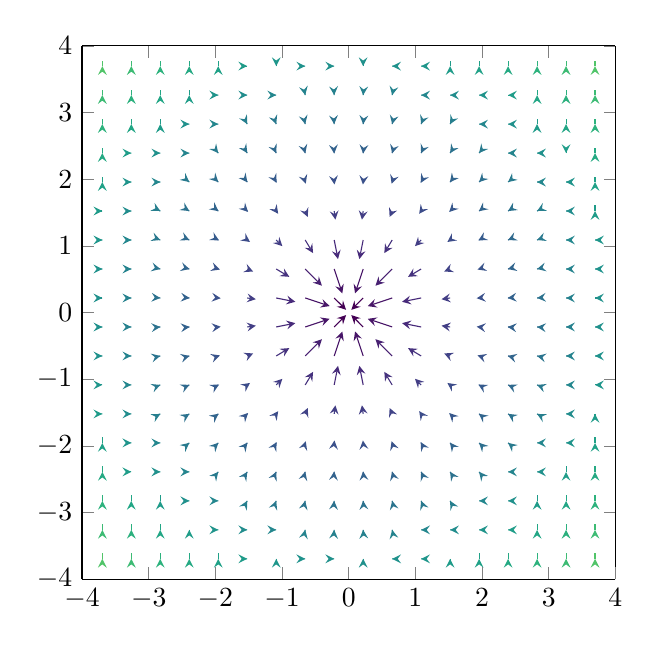
\begin{tikzpicture}
      \begin{axis}[%
         xmin = -4, xmax = 4,
         ymin = -4, ymax = 4,
         zmin = 0, zmax = 1,
         axis equal image,
         xtick distance = 1,
         ytick distance = 1,
         view = {0}{90},
         scale = 1.25,
         height=7cm,
         colormap/viridis,
      ]
      \addplot3[point meta = {sqrt(x^2+y^2)}, quiver={u=-2*x*exp(-x^2-y^2), v=-2*y*exp(-x^2-y^2), scale arrows=0.45}, quiver/colored = {mapped color}, samples=24, -stealth] (x,y,0);
     \end{axis}
   \end{tikzpicture}
   \captionsetup{labelformat=empty}
   \caption{Gradient de la fonction \(f : (x, y) \mapsto \exp(-x^2 - y^2)\)}
\end{figure}
Une autre propriété remarquable du gradient est qu'il est toujours \textbf{orthogonal} aux lignes de niveaux.

\subsection*{\subsecstyle{Caractérisation des dérivées directionnelles{:}}}
Pour un vecteur unitaire \(v\) donné, on peut alors montrer la caractérisation trés utile de la dérivée directionelle de \(f\) dans la direction de \(v\), en effet on a:
\[
   D_vf(a) = df_a(v) = \dotproduct{\nabla f(a)}{v}  
\]
En effet, il suffit alors d'écrire la formule de Taylor à l'ordre 1 sur la quantité ci-dessous et utiliser les différentes propriétés des objets considérés:
\[
   f(a + hv) - f(a) = df_a(hv) + o(\vectNorm{hv})
\]
\uline{Exemple:} Pour \(f(x,y) = xy + x\) et  \(v = \frac{1}{\sqrt{2}}(1, 1)\) alors on a:
\[
   df_{(x, y)} = (y+1)dx + xdy   
\]
Et donc finalement:
\[
   D_vf(x, y) = \frac{1}{\sqrt{2}}(y + x + 1)
\]
On peut remarque que si on prends \(v = e_i\), on retombe évidemment sur les dérivées partielles.
\pagebreak

\subsection*{\subsecstyle{Jacobienne{:}}}
On considère maintenant plus généralement l'espace des fonctions de classe \(\mathcal{C}^1(\R^n, \R^p)\), et on définit alors l'opérateur suivant:
\[
   \begin{aligned}
      J : \mathcal{C}^1(\R^n, \R^p) &\longrightarrow \mathcal{M}_{p, n}(\mathcal{F}(\R^n, \R^p))\\
      f &\longmapsto \begin{pmatrix}
         \partialD{f_1}{x_1} &\ldots &\partialD{f_1}{x_n}\\
         \vdots &\ddots &\vdots \\ 
         \partialD{f_p}{x_1} &\ldots &\partialD{f_p}{x_n}
      \end{pmatrix}
   \end{aligned}
\]
On appellera alors \textbf{jacobienne} de \(f\) la matrice \(Jf\), et on remarque que c'est simplement la matrice\footnote[1]{A coefficients dans l'anneau des fonctions.} constituée des dérivées partielles de \(f\).\<

En particulier, on a donc l'identité suivante:
\[
   Jf = \begin{pmatrix}
      \nabla f_1\\
      \vdots\\ 
      \nabla f_n
   \end{pmatrix}
\]
\begin{center}
   \textit{C'est aussi la matrice des gradients des applications partielles de \(f\).}
\end{center}
Si on l'évalue maintenant en un point \(a \in \R^n\), on obtient alors une matrice réelle et on a la caractérisation fondamentale suivante:
\begin{center}
   \textbf{La jacobienne prise en un point est la matrice de la différentielle en ce point.}
\end{center}
En particulier on retrouve donc la règle de la composition de la différentielle vu sous l'angle matriciel:
\[
   J(f \circ g)_a = Jf_{g(a)} \times Jg_{g(a)}
\]
Ainsi que la règle de l'inversion d'une fonction inversible:
\[
   (Jf_{a})^{-1} = J(f^{-1})_{f(a)}
\]
\chapter*{\chapterstyle{VII --- Théorèmes généraux}}
\addcontentsline{toc}{section}{Théorèmes généraux} 
Dans cette section, nous allons utiliser toutes les notions construites au chapitre précédent pour essayer de généraliser les grands théorèmes sur les fonctions réelles dérivables, en particulier les deux théorèmes suivants:
\begin{itemize}
   \item Le théorème de la bijection
   \item Le théorèmes des accroissements finis
\end{itemize}
Le problème principal pour obtenir un analogue au premier théorème est le suivant:
\begin{center}
   \textit{Il existe des fonctions non-injectives telles qu'en tout point leur différentielle soit inversible !}
\end{center}
Ce qui implique alors que nous ne pouvons pas prouver l'injectivité \textbf{globale} d'une fonctions à plusieurs variables avec le critère simple de la non-annulation de la différentielle. Ceci nous menera donc à la recherche de théorème permettant de montrer la bijectivité de ces fonctions autrement.

\subsection*{\subsecstyle{Théorème d'inversion locale{:}}}
On considère \(f : \R^n \longrightarrow \R^p\) de classe \(\mathcal{C}^1\) et un point \(a \in \R^n\), alors si sa différentielle est \textbf{inversible} en \(a\), on a:
\begin{center}
   \textbf{La fonction induit un \(\mathcal{C}^1\)-difféomorphisme d'un voisinage \(V_a\) dans \(f(V_a)\).}
\end{center}
On peut interpréter ce théorème de manière plus naturelle sous la forme:
\begin{center}
   \textit{Si la différentielle ne s'annule pas en un point, alors la fonction est localement inversible en ce point.}
\end{center}

\subsection*{\subsecstyle{Théorème d'inversion globale{:}}}
On considère \(f : \R^n \longrightarrow \R^p\) une fonction \textbf{injective} et de classe \(\mathcal{C}^1\), alors si en tout point d'un ouvert \(\mathcal{U}\) sa différentielle est \textbf{inversible}, on a:
\begin{center}
   \textbf{La fonction induit un \(\mathcal{C}^1\)-difféomorphisme de \(\mathcal{U}\) sur \(f(\mathcal{U}).\)}
\end{center}
On peut interpréter ce théorème de manière plus naturelle sous la forme:
\begin{center}
   \textit{Sous réserve d'injectivité, si la différentielle ne s'annule pas sur un ouvert, alors la fonction est inversible sur cet ouvert.}
\end{center}

\subsection*{\subsecstyle{Théorème des fonctions implicites{:}}}
On considère une fonctions \(f : \R^n \rightarrow \R\) de classe \(\mathcal{C}^1(\R^n)\) et on s'intéresse aux courbes \(\Gamma\) d'équation:
\[
   f(x_1, \ldots, x_n) = 0   
\]
Si il est possible d'exprimer une variable en fonction des autres, ie d'isoler une variable \(x_i\), alors on dira que l'équation \(E\) définit \(x_i\) comme \textbf{une fonction implicite} des \(n-1\) autres variables. On s'intéresse ici à des condition suffisantes sur \(f\) pour que de telles fonctions implicites existent.\<

On peut alors montrer gràce au \textbf{théorème d'inversion locale} que si \((x_1, \ldots, x_n) \in \Gamma\), et que la \(i\)-ème dérivée partielle ne s'annule pas, alors \textbf{localement} l'équation définit bien \(x_i\) comme fonction implicite des \(n-1\) autres variables pour un certaine fonction \(\phi\) de classe \(\mathcal{C}^1(\R^{n-1})\), ie on a:
\[
   x_i = \phi(x_1, \ldots, x_{i-1}, x_{i+1}, \ldots, x_n)   
\]
Prenons un exemple simple pour illustrer le propos
\pagebreak

On considère la courbe \(\Gamma\) suivante:
\[
   f(x,y) = x^2 + y^2 - 1 =0
\]
On reconnaît immédiatement le cercle unité, le théorème des fonctions implicites affirme alors qu'à l'exception des points \((\pm 1, 0)\), cette équation définit implicitement \(y\) comme une fonction de \(x\) et en effet, on sait que par exemple dans le demi-plan supérieur, on a:
\[
   y = \sqrt{1 - x^2}   
\]
Ce théorème justifie une technique courante dans la littérature anglo-saxonne nommé \textbf{différentiation implicite}, en effet si on considère une équation d'un fonction à deux variables (par exemple), alors on peut "voir"\footnote[1]{Sous les hypothèses de régularité du théorème bien évidemment.} une des variables comme fonction de l'autre et simplement différentier, et par exemple on peut de cette manière trouver les dérivées des fonctions réciproques:
\begin{flalign*}
   y = \cos^{-1}(x) &\Longleftrightarrow \cos(y) = x\\
   &\Longleftrightarrow \sin(y)y' = -1  \shorteqnote{(On "voit" \(y\) comme fonction de \(x\) et on différentie.)}\\
   &\Longleftrightarrow y' = \frac{-1}{\sin(y)}\\
   &\Longleftrightarrow y' = \frac{-1}{\sin(\cos^{-1}(x))}\\
   &\Longleftrightarrow y' = \frac{1}{-\sqrt{1-x^2}}
\end{flalign*}

\subsection*{\subsecstyle{Théorème des accroissements finis{:}}}
On considère ici un champs scalaire\footnote[2]{Il n'existe pas d'équivalent au théorème des accroissements finis dans le cas de fonctions à valeurs vectorielles, considérer par exemple la courbe \(t \mapsto (\cos(t), \sin(t))\).} défini et différentiable sur un ouvert \(\mathcal{U}\), alors pour tout point \(a, b \in \mathcal{U}\) tel que le segment \([a, b]\) les reliant soit dans \(\mathcal{U}\), on a\footnote[3]{La démonstration de cette propriété revient à se ramener au cas réel en posant \(g(t) = f((1 - t)a + tb)\)}:
\[
   \exists c \in \mathcal{U} \; ; \; f(b) - f(a) = df_c(b - a)   
\]
En particulier si \(\mathcal{U}\) est convexe, cette propriété est vrai pour tout couple \((a, b)\).

\subsection*{\subsecstyle{Corollaire 1 : Inégalité des accroissements finis{:}}}
En particulier, si la différentielle \(df_x\) est \textbf{bornée} par un réel \(M\) sur \(\mathcal{U}\), alors on a aussi:
\[
   |f(b) - f(a)| \leq M(b - a)
\]
Cette majoration reste vraie, contrairement au théorème, dans le cas de champs de vecteurs et on a alors pour des normes bien choisies:
\[
   \vectNorm{f(b) - f(a)} \leq M\vectNorm{b - a}
\]
En particulier, cela montre donc que les applications différentiables sont toutes \textbf{localement} lipschitziennes, et même globablement lipschitziennes si la différentielle est bornée.

\subsection*{\subsecstyle{Corollaire 2 : Applications constantes {:}}}
On peut alors généraliser le critère des fonctions réelles qui nous affirme que si la dérivée d'une fonction est nulle, elle est constante. En effet, si \(f : \mathcal{U} \rightarrow \R\) différentiable sur \(\mathcal{U}\) ouvert et \textbf{connexe}\footnote[4]{La preuve est directe si \(\mathcal{U}\) est convexe, pour passer à la connexité, il faut alors remarque que toutes les boules sont convexes.}, alors:
\begin{center}
   Si la différentielle de \(f\) est \textbf{nulle} sur \(\mathcal{U}\), alors \(f\) est \textbf{constante} sur \(\mathcal{U}\).
\end{center}

\subsection*{\subsecstyle{Corollaire 3 : Applications constantes par rapport à une variable {:}}}
On s'intéresse alors à ce qu'on peut déduire de l'annulation d'une seule des dérivées partielles, et en se ramenant à l'étude des application partielles on peut alors montrer que si \(f : \mathcal{U} \rightarrow \R\) différentiable sur \(\mathcal{U}\) ouvert et \textbf{convexe}\footnote[2]{\textbf{ATTENTION:} Ce résultat est faux sur un domaine juste connexe. Prendre la fonction qui définie sur \(\R^2\) privée d'un axe bien choisi qui vaut \(0\) sur \(\{ (x, y), xy < 0\}\) et \(x^2\) ailleurs.} et que \(\partialD{f}{x_i}\) est \textbf{nulle} sur \(\mathcal{U}\), alors il existe une fonction \(g\) telle que:
\[
   \forall (x_1, \ldots, x_n) \in \mathcal{U} \; f(x_1, \ldots, x_n) = g(x_1, \ldots, x_{i-1}, x_{i+1}, \ldots, x_n) 
\]
\begin{center}
   \textit{Intuitivement, on l'interprète simplement par le fait que \(f\) ne dépends pas de la variable \(x_i\) sur cet ouvert.}
\end{center}
C'est ce corollaire qui nous permettra de résoudre nos premières équations aux dérivées partielles. Voici un exemple élementaire, on considère une fonction \(f\) de classe \(\mathcal{C}^1(\R^2)\) qui vérifie:
\[
   \partialD{f}{x}(x, y) = 0   
\]
Alors d'aprés ce corollaire, on a directement, pour \(g \in \mathcal{C}^1(\R)\) une certaine fonction réelle:
\[
   f(x, y) = g(y)   
\]

\chapter*{\chapterstyle{VII --- Optimisation I}}
\addcontentsline{toc}{section}{Optimisation I} 
Un des intérets de la notion de dérivée d'une fonction réelle est de pouvoir étudier les extrema de cette fonction, en particulier, un point capital du cours d'analyse réelle est la définition de \textbf{point critique}, qui sont les points d'annulation de la dérivée, et on a alors la condition nécessaire suivante:
\begin{center}
   \textbf{Si un point est un extremum, alors c'est un point critique.}
\end{center}
On veut généraliser cette notion au cas des \textbf{champs scalaires}, pour à terme être capable de trouver les extrema de telles fonctions.

\subsection*{\subsecstyle{Points critiques{:}}}
De manière parfaitement analogue, si \(f\) est une fonction définie sur un ouvert \(\mathcal{U}\), alors on définit les \textbf{points critiques}, qui sont les points d'annulation de la différentielle, et on a alors la condition nécessaire suivante:
\begin{center}
   \textbf{Si un point est un extremum, alors c'est un point critique.}
\end{center}
Informellement, on comprends naturellement que les seuls extrema possibles seront ceux où l'application linéaire tangente est nulle, donc un plan horizontal. Néanmoins la condition n'est que nécessaire, en effet on considère la fonction:
\[
   f : (x, y) \mapsto xy   
\]
Alors sa différentielle est nulle en \((0, 0)\), mais ce point n'est pas un extremum, il suffit d'étudier quelques restrictions pour le montrer. On a donc besoin d'outils plus puissants pour trouver ces extrema. 
\subsection*{\subsecstyle{Hessienne{:}}}
On suppose maintenant que \(f \in \mathcal{C}^2(\R^n)\), alors elle admet toutes ses dérivées partielles secondes et elle vérifie le \textbf{théorème de Schwarz}. On définit alors la \textbf{matrice Hessienne} de \(f\) par:
\[
   \mathcal{H}f_{(x, y)} = \left(\partialD{{}^2f}{x_ix_j}\right)_{i ,j \in \inticc{1}{n}} = 
   \begin{pmatrix}
      \partialD{{}^2f}{x_1^2} & \ldots & \partialD{{}^2f}{x_1x_{n}}\\ 
      \vdots & \ddots & \vdots\\ 
      \partialD{{}^2f}{x_{1}x_n} & \ldots & \partialD{{}^2f}{x_{n}^2}\\   
   \end{pmatrix}   
\]
Cette matrice est \textbf{symétrique} d'aprés le théorème de Schwarz, elle définit donc une forme bilinéaire symétrique et une forme quadratique, qu'on appelera forme hessienne, qui jouera un rôle important pour la suite.
\subsection*{\subsecstyle{Classification des points critiques{:}}}
Dans le cas réel, pour classifier les points critiques d'une fonction, on étudiait la convexité (locale) de cette fonction, et en particulier le signe de la dérivée seconde, ceci permettait de différencier les maxima, minima et point cols (ou point d'inflexions). D'une certaine manière, on généralise cette approche au cas général en étudiant \textbf{le signe de la Hessienne} au sens du signe d'une forme quadratique, et on a les cas suivants:
\begin{itemize}
   \item Si la forme hessienne n'est \textbf{ni positive ni négative} en un point critique, alors le point est un \textbf{point col}.

   \item Si la forme hessienne est \textbf{définie positive} en un point critique, alors la fonction est localement convexe et le point est un \textbf{minimum}.
   \item Si la forme hessienne est \textbf{définie négative} en un point critique, alors la fonction est localement concave et le point est un \textbf{maximum}.
   \item Sinon la méthode ne permet pas de conclure.
\end{itemize}
On se ramène donc à l'étude des valeurs propres de la Hessienne, et de leurs signes ou dit autrement, de la signature de la forme quadratique Hessienne. Ceci s'interprète en disant que, de manière analogue au cas réel, le signe de la hessienne caractérise la \textbf{convexité locale} de la fonction.
\chapter*{\chapterstyle{VII --- Optimisation II}}
\addcontentsline{toc}{section}{Optimisation II} 
Pour aller plus loin, on peut s'intéresser à essayer d'optimiser une fonction \( f : \R^n \longrightarrow \R \) sous la contrainte que \(x \in \left\{ x \in \R^n \; ; \; g(x) = 0 \right\}\) où \( f, g \) sont lisses et où \( g \) satisfait les conditions du théorème des fonctions implicites (ie que \( dg \) soit de rang maximal, partout pour simplifier). En d'autres termes on veut résoudre le problème d'optimisation suivant:
\[ 
   (P) :\begin{cases}
      \sup f(x)\\
      x \in C := \left\{ x \in \R^n \; ; \; g(x) = 0 \right\} 
   \end{cases} 
\] 
On cherche alors une méthode permettant de résoudre un tel problème, et plus particulièrement une méthode permettant de passer de ce problème à un \textbf{problème d'optimisation sans contraintes}.
\subsection*{\subsecstyle{Conditions nécéssaires {:}}}
On considère un point \( x \in \R^n \) qui est solution du problème, et \( v \) un vecteur \textbf{tangent} à \( \left\{ x \in \R^n \; ; \; g(x) = 0\right\}\), alors on peut montrer que nécessairement:
\[ 
   df_x(v) = 0 \iff \dotproduct{\nabla f(x)}{v} = 0
\]
Ce qui s'interprète alors par le fait que \( \nabla f_x \) est \textbf{orthogonal} à l'espace tangent à \( \left\{ x \in \R^n \; ; \; g(x) = 0\right\} \), or celui ci (par le théorème des fonctions implicites) peut localement s'écrire comme:
\[ 
   \left\{ x \in \R^n \; ; \; \dotproduct{\nabla g(x)}{x} = 0\right\} =  \left\{ \nabla g(x) \right\}^\perp 
\]
Finalement on trouve alors que \( f \) est orthogonale à un orthogonal et donc colinéaire au \textbf{gradient de la contrainte}, ie on a:
\[ 
   \exists \lambda \in \R \; ; \; \nabla f(x) = \lambda\nabla g(x) 
\]
Plus généralement, si on a \( m \) contraintes données par des fonction \( g_i \), on a;
\[ 
   \exists (\lambda_i) \in \R^m \; ; \; \nabla f(x) = \sum_{i=1}^m \lambda_i \nabla g_i(x) 
\]
\subsection*{\subsecstyle{Lagrangien {:}}}
On encapsule alors toutes les contraintes du problème en posant la fonction suivante appellée \textbf{lagrangien} du problème:
\[ 
   \mathcal{L}(x, \lambda) = f(x) + \dotproduct{\lambda}{g(x)} 
\]
Alors c'est une fonction lisse de ses variables et si \( x \) est solution du problème, on montre que l'on a nécessairement:
\[ 
   \nabla \mathcal{L}(x, \lambda) = 0
\]
Cette fonction nous donne alors une condition \textbf{nécessaire} que doit vérifier un extremum sous contrainte.
\subsection*{\subsecstyle{Méthode d'optimisation {:}}}
On peut donc construire une méthode qui permet de résoudre de tels problèmes. En effet, on peut appliquer l'algorithme suivant:
\begin{itemize}
   \item On cherche à montrer \textbf{l'existence} d'un extermum sous contraintes (par exemple par compacité de \( C \)).
   \item On calcule les \textbf{points critiques du Lagrangien} qui sont alors tout les \textbf{candidats} possibles.
\end{itemize}

\chapter*{\chapterstyle{VII --- Formes différentielles}}
\chapter*{\chapterstyle{VII --- Intégrales Curvilignes}}
\addcontentsline{toc}{section}{Intégrales Curvilignes} 

Dans cette partie, nous allons généraliser l'intégrale de Riemann, c'est à dire l'intégrale d'une fonction le long d'un segment, aux \textbf{champs scalaires et vectoriels}, avec en tête l'idée suivante:
\begin{center}
   \textit{On veut pouvoir intégrer un champ le long d'une courbe lisse donnée.}
\end{center}
Nous verrons alors qu'il existe en fait trois constructions différentes qui mesurent différents phénomênes sur les champs considérés:
\begin{itemize}
   \item L'intégrale d'un \textbf{champ scalaire} qui quantifie l'aire entre la courbe et le plan des paramétres.
   \item L'intégrale de \textbf{travail} d'un \textbf{champ vectoriel} qui quantifie la contribution du champ vectoriel au trajet de la courbe.
   \item L'intégrale de \textbf{flux} d'un \textbf{champ vectoriel} qui quantifie la tendance au champ de vecteurs à traverser la courbe.
\end{itemize}
Dans toute la suite, on considèrera un \textbf{arc orienté} \(\Gamma\) paramétré par une fonction \(\gamma : t \mapsto \gamma(t)\) définie sur \(\icc{a}{b}\) et de classe \(\mathcal{C}^1\). On rapelle à toutes fins utiles:
\begin{itemize}
   \item L'abcisse curviligne de \(\gamma\) est donnée par: \(ds = \vectNorm{\gamma'(t)} d t  \)
   \item Le vecteur normal à \(\gamma'\) est donnée par: \(dn = (\gamma_2'(t), -\gamma_1'(t))d t  \)
\end{itemize}
\subsection*{\subsecstyle{Intégrale d'un champ scalaire{:}}}
On se donne un champ scalaire lisse \(f : \Gamma \rightarrow \R\) et on cherche à quantifier l'aire située entre la courbe et le graphe \(\mathscr{G}_f\), on peut alors écrire cette aire comme une somme de Riemann, qui tends alors vers une intégrale et on définit:
\[
   \int_{\gamma} f d s = \int_{a}^{b}f(\gamma(t))\vectNorm{\gamma'(t)}d t
\]
\subsection*{\subsecstyle{Intégrale de travail d'un champ vectoriel{:}}}
On se donne un champ vectoriel lisse \(f : \Gamma \rightarrow \R^n\) et on cherche à quantifier la \textbf{contribution du champ vectoriel au trajet de la courbe}, ie au travail que le champ effectuerais sur une particule qui se déplacerait le long de la courbe, à nouveau gràce aux sommes de Riemann, on peut définir:
\[
   \int_{\gamma} F d \gamma = \int_{a}^{b} \dotproduct{F(\gamma(t))}{\gamma'(t)}dt
\]
\subsection*{\subsecstyle{Intégrale de flux d'un champ vectoriel{:}}}
On se donne un champ vectoriel lisse \(f : \Gamma \rightarrow \R^n\) et on cherche à quantifier la \textbf{tendance au champ de vecteurs à traverser la courbe}, ie si le champ de vecteurs représenterais un fluide, à la quantité d'eau qui traverse la courbe en un instant donné. A nouveau gràce aux sommes de Riemann, on peut définir:
\[
   \int_{\gamma} F d n = \int_{a}^{b} \dotproduct{F(\gamma(t))}{n'(t)}d t
\]
\subsection*{\subsecstyle{Intprétation du produit scalaire{:}}}
On remarque que les intégrales curviligne d'un champ de vecteur font apparaître un produit scalaire, en effet cela déocule directement des quantités géométriques que l'on cherche à calculer:
\begin{itemize}
   \item Dans le cas d'une intégrale de travail, on considère la projection d'un vecteur du champ sur un vecteur tangent, c'est \textbf{la composante tangentielle} du champ, et on somme toutes ses composantes pour obtenir une contribution totale.
   \item Dans le cas d'une intégrale de flux, on considère la projection d'un vecteur du champ sur un vecteur normal, c'est \textbf{la composante normale} du champ, et on somme toutes ses composantes pour obtenir une contribution totale mais dans un autre sens.
\end{itemize}
\subsection*{\subsecstyle{Théorème du gradient{:}}}
On s'attarde un peu sur le cas vectoriel, et on se donne un champ vectoriel \(X\) tel que \(X = \nabla F\) pour un certain champ scalaire \(F\), on dira alors que \(X\) \textbf{dérive du potentiel} \(F\), on se donne un chemin paramétré par \(\gamma\) sur \(\icc{a}{b}\) et on cherche à calculer le travail de \(X\) sur ce chemin, on trouve alors que:
\begin{flalign*}
   \int_{\gamma} X d \gamma &:= \int_{a}^{b} \dotproduct{\nabla F(\gamma(t))}{\gamma'(t)}d t \\
   &= \int_{a}^{b} dF_{\gamma(t)}(\gamma'(t)) d t \shorteqnote{(On utilise le lien gradient / différentielle.)} \\ 
   &= \int_{a}^{b} d(F \circ \gamma)_t \shorteqnote{(Par la règle de la chaîne, ou en passant en composantes.)}  \\ 
   &= \int_{a}^{b} (F \circ \gamma)'(t) d t \shorteqnote{(Par le lien diférentielle / dérivée.)}  \\ 
   &= F(\gamma(b)) - F(\gamma(a)) \shorteqnote{(Théorème fondamental de l'analyse.)}  \\ 
\end{flalign*}
En particulier, on a montré le théorème suivant, généralisation du théorème fondamental de l'analyse, appelé souvent \textbf{théorème du gradient}:
\begin{center}
   \textbf{Le travail le long d'un chemin d'un champ qui dérive d'un potentiel ne dépends que des bords du chemin choisi.}
\end{center}
C'est en fait même un cas particulier d'un théorème trés général qu'on verra plus tard apellé \textbf{théorème de Stokes} qui affirme que pour une forme différentielle \textbf{exacte}, ie qui s'écrive \(d\omega\) pour \(\omega\) une autre forme différentielle, alors on a que l'intégrale ne dépends que des bords:
\[
   \int_{A} d \omega = \int_{\partial A} \omega
\]
\subsection*{\subsecstyle{Généralisations{:}}}
On imagine alors qu'il doit être possible de généraliser ces concepts d'intégrales sur une courbe (espace de dimension 1) à des intégrales sur des \textbf{surfaces, volumes ...}. On aurait alors les deux\footnote[1]{Le concept d'intégrale de travail ne se généralise pas conceptuellement aux dimensions plus grandes pour des raisons évidentes.} concepts géométriques suivants:
\begin{itemize}
   \item L'intégrale sur une surface d'un \textbf{champ scalaire} qui quantifierait le volume entre la courbe et le plan des paramétres.
   \item L'intégrale sur une surface d'un \textbf{champ vectoriel} qui quantifierait la tendance au champ de vecteurs à traverser la surface.
\end{itemize}
\chapter*{\chapterstyle{VII --- Intégrales Multiples}}
\addcontentsline{toc}{section}{Intégrales Curvilignes} 
Dans ce chapitre on cherche à généraliser la notion d'intégrale d'une fonction d'une seule variable sur un segment à la notion d'intégrale d'une fonction réelle \textbf{de plusieurs variables qu'on supposera bornée}, ici on considérera principalement \(f : \R^2 \rightarrow \R\) pour simplifier l'exposition. On a alors deux nouveaux concepts d'intégrales qui se présentent:
\begin{itemize}
   \item La notion d'intégrale \textbf{curviligne} qui se propose d'intégrer à nouveau sur un chemin (donc toujours sur un espace de dimension 1).
   \item La notion d'intégrale \textbf{multiple} qui se propose d'intégrer sur une surface (donc sur un espace de dimension plus grande).
\end{itemize}
Ces deux notions différentes coexistent et permettent de résoudre des problèmes trés différents, nous nous proposons ici tout d'abord de définir la notion d'intégrale multiple. Moralement, l'idée consiste à se donner un domaine raisonnable \(\mathcal{D}\) de \(\R^2\), et de chercher à calculer le \textbf{volume} au dessus \(\mathcal{D}\) et contenu sous la nappe définie par l'image de \(f\). 

Graphiquement, voila ce que l'on cherche à réaliser, ici le domaine d'intégration étant un simple rectangle:
\begin{center}
   \begin{tikzpicture}[
      x=(215:2em/sqrt 2), y=(0:2em), z=(90:2em),
      declare function={f(\x,\y)=((\x-3)^2+(-\y+3)^3)/8+3;}, 
      very thick, line join=round]
    \draw [-stealth, black!75] (0,0,0) -- (6,0,0) node [below left] {$x$};
    \draw [-stealth, black!75] (0,0,0) -- (0,6,0) node [below right] {$y$};
    \draw [-stealth, black!75] (0,0,0) -- (0,0,6) node [right] {$z$};
    \foreach \x in {1,...,4}
      \foreach \y [evaluate={\j=\x+.5; \i=\y+.5; \k=f(\j,\i);}] in {1,...,4}{
        \path [fill=DarkBlue2!50, draw=white] (\x, \y+1, 0) -- (\x+1, \y+1, 0) -- 
          (\x+1, \y+1, \k) -- (\x, \y+1, \k) -- cycle;
        \path [fill=DarkBlue2!25, draw=white] (\x+1, \y, 0) -- (\x+1, \y+1, 0) -- 
          (\x+1, \y+1, \k) -- (\x+1, \y, \k) -- cycle;
        \path [fill=DarkBlue2!10, draw=white] (\x, \y, \k)  -- (\x+1, \y, \k) -- 
          (\x+1, \y+1, \k) -- (\x, \y+1, \k) -- cycle;
      }
     \foreach \x in {1,...,4}
       \foreach \y in {1,...,4}{
     \draw [DarkBlue2, fill=DarkBlue2, fill opacity=0.125, 
        domain=0:1, samples=20, variable=\t] 
        plot (\x+\t, \y, {f(\x+\t,\y)}) -- 
        plot (\x+1, \y+\t, {f(\x+1,\y+\t)}) -- 
        plot (\x+1-\t, \y+1, {f(\x+1-\t,\y+1)}) --
        plot (\x, \y+1-\t, {f(\x,\y+1-\t)}) -- cycle;
      }


    \end{tikzpicture}
\end{center}

\subsection*{\subsecstyle{Outils préliminaires{:}}}
On souhaite intégrer \(f\) sur le rectangle \(R = [a, b] \times [c, d]\), on considère alors une \textbf{subdivision} de \(R\) c'est à dire un couple de subdivisions de \([a, b] \text{ et } [c, d]\) respectivement, ie on se donne \((a = t_0, t_1, \ldots, t_{n-1}, t_n = b)\) et \((c = t'_0, t'_1, \ldots, t'_{n-1}, t'_n = d)\), alors ces subdivisions définissent des \textbf{sous-rectangles} par:
\[
   R_ij = [t_i, t_{i+1}] \times [t'_j, t'_{j+1}]   
\]
On appellera la collection de ces sous-rectangles une \textbf{subdivision} du rectangle \(R\). On définit de manière évidente le \textbf{volume} (ici une aire) d'un rectangle \(R\) par:
\[
   \text{Vol}(R) = (b - a)(d - c) 
\]
Finalement on définit aussi les deux quantités suivantes pour tout rectangle \(R\):
\[
   \begin{cases}
      m_R(f) &:= \left\{ \inf(f(x)) \, ; \, x \in R \right\}\\
      M_R(f) &:= \left\{ \sup(f(x)) \, ; \, x \in R \right\}
   \end{cases}   
\]
\pagebreak
\subsection*{\subsecstyle{Intégrale sur un rectangle{:}}}
Soit \(R\) le rectangle domaine d'intégration et \(P\) une subdivision de \(R\), alors on définit les \textbf{sommes de Darboux supérieure et inférieures} par:
\[
   \begin{cases}
      S_P^+(f) = \sum_R M_R(f) \cdot \text{Vol}(R)\\
      S_P^-(f) = \sum_R m_R(f) \cdot \text{Vol}(R) 
   \end{cases}
\] 
Où la somme parcourt tout les rectangles de la subdivision. On définit alors les \textbf{intégrales de Darboux supérieure et inférieures} par:
\[
   \begin{cases}
      \displaystyle\int_R^+{f} = \inf\left\{\, S_P^+(f)\; ; \; P \text{ est une subdivision de } R\right\}\\
      \displaystyle\int_R^-{f} = \sup\left\{\, S_P^-(f)\; ; \; P \text{ est une subdivision de } R\right\}
   \end{cases}
\]
\begin{center}
   \textit{
      L'intégrale supérieure (resp. inférieure) est la somme \textbf{minimale} (resp. maximale) obtenue en considérant \textbf{toutes les subdivisions possibles} du rectangle.
   }
\end{center}
Enfin on dit que \(f\) est \textbf{intégrable} sur \(R\) si et seulement si \textbf{l'intégrale supérieure et inférieure} sont égales, et on la note formellement:
\[
   \int_R f d x_1 \ldots d x_n \overset{\text{def.}}{=} \int_R f 
\]


\subsection*{\subsecstyle{Intégrale sur un ensemble borné{:}}}


.... -> Admettons pour le moment que l'on sait intégrer sur des surfaces ...
